\chapter{Literature Review}

Except the initial work done by Axelrod, there are many other papers that have tried
to tangle the game of PD and make their conclusions on cooperation in
both theoretical and real life behavior. In this chapter we review some of this work
done in the IPD competitions, in spatial and evolutionary game theory.

\section{The Prisoner's Dilemma}
The PD was originally formulated by Merril M. Flood and Melvin Dresher,
who were working on the Flood-Desher Experiment at the RAND cooperation in 1950.
Later in 1950, the mathematician Albert W. Tucker presented the first formal
representation of the PD, titled  A Two-Person Dilemma in a seminar at
Stanford University\parencite{Gass005}.

A description of the PD, found in \parencite{Li2011} is as follows :
There are two players that simultaneously have to decide to whether Cooperate(C)
or Defect (D) with each other, without exchanging informations.

\begin{itemize}
  \item If both players choose to cooperate they will both receive a reward (R)
  \item If a player defects and the other cooperates then the defector receives
  a temptation payoff (T) and the cooperator a sucker payoff (S)
  \item If both players defect they will both receive a penalty (P)
\end{itemize}

Fig. 1 illustrates the payoffs matrix.~\ref{fig:pd_payoff}.

\begin{figure}[h!]
\centering
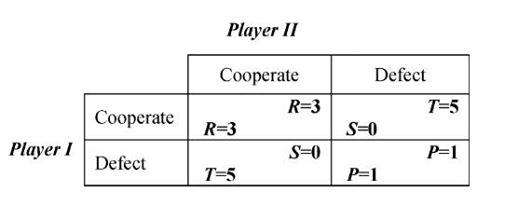
\includegraphics[scale=0.45]{pd_payoff.jpg}
\caption{Prisoner's Dilemma Payoff Matrix.\parencite{Li2011}}
\label{fig:pd_payoff}
\end{figure}

Taking into account the assumptions that both players are both rational human beings and
that there is no way of communication between them,it can be shown that in the standard
form of the PD a pure Nash Equilibrium exists when both players defect.
So the outcome of any one round game will be Defection.

The Prisoner’s Dilemma can also be studied for any given number of iterations(IPD)
, where players play each other repeatedly. An extra condition for the payoffs
in the IPD are : T \(>\) R \(>\) P \(>\) S and R \(>\) 1/2(T+S).

\section{Tournaments}

In 1980, Robert Axelrod held two computer tournaments based on the game Iterated
Prisoner's Dilemma as descripted above. In the first tournament 14 different
strategies written by scientists from different fields competed each other on a
tournament of 200 turns per game and in a round robin topology. Axelrod also added
two more strategies : a Random one and a Twin.

A strategy called Tit for Tat was announced the winner of the first tournament.
Tit for Tat is a deterministic strategy that will always cooperate in the first
round and afterwards it copies the opponents last move. Surprisingly in the second
tournament held by Axelrod \parencite{Axelrod1980a} where 64 strategies competed and all they
writes had full knowledge of what have happened in the first tournament, Tit
for Tat managed to get first place again.

As explained by Axelrod \parencite{Axelrod1980b}, Tit for Tat a simple strategy was able to
win the rest of sophisticated and more complex strategies based on three specific
characteristics of the strategy :
\begin{itemize}
  \item Niceness :  A strategy is categorized as nice if it was not the
                    first to defect , or at least, it will not do this until
                    the last few moves.
  \item Forgiveness : The propensity to cooperate in the moves after the
                      opponent defected.
  \item  Clarity : After opponents identified that they were playing Tit for Tat
                  choose to cooperate for the rest of the game.
\end{itemize}

The first tournaments were an innovation in combining computer modeling and
Game Theory and in providing insights in the behavior emerging from simple dynamics.
Moreover, Axelrod was the first to have spoken about niceness , forgiveness and have given proof
that cooperation can be a victorious and advantageous strategy.

Add more tournaments and criticisms on Axelrod's work.

\section{Spatial Structure Tournaments}

Nowak and May in 1992, were the first ones that conducted a PD tournament using
spatial structure\parencite{Nowak_&_May1992}. Their tournament was a simple and
purely deterministic spatial version of the PD, with no memories among the
players and no strategical elaboration, they players could  either always
cooperate or defect. Most of the work done by various other authors are only
using these two basic strategies. These trials on the spatial tournament were the
perfect tool to identify the effect that a different topology than a round robin would have
on previous studies. Indeed,  Nowaw and May manage to show that such structure
has an important effect as it was shown that cooperation could merge for the simple PD.

Similarly, in 1994 Lindgren and Nordahl\parencite{Lindgren_&_Nordahl1994} inspired by the work
done by Nowak and May decided to run their own tournament. This time though the would use the
IPD, allowing players to keep memory and therefore adding a bit more complex strategies to the
tournament such as Tit for Tat and  Anti Tit for Tat. Followed  by the work of
\parencite{Brauchli_&_Killingback_&_Doebelis1999}
 which introduced even more complex strategies.

Furthermore, in the first tournament tournament the spatial structure is defined
as an 2D square lattice where players can only play their von Neuman or Moore neighbors.
A lattice is defined as a graph, but
in non paper the author has defined a spatial structure as graph, expect from
\parencite{Meng&Xia_etc2015} where they defined it as a network.

Another interesting aspect of spatial IPD games is evolution. Nowak and May, in both
their paper used a deterministic approach, such as the player in a neighborhood
would mirror the move of the neighbor with the highest payoff of all.
An interesting approach in evolute was given by \parencite{Meng&Xia_etc2015}
where they used a two lattices topology  and a player would mimic a random player
base on a function that consider the utility of the player. Where each player’s
utility will not only consider his/her own payoff, but also incorporate the
payoff of corresponding partner from the other lattice.

\section{Evolution and Moran process}

\section{Axelrod Python Library}

The Axelrod library is an open source Python package that allows for
reproducible game theoretic research into the Iterated Prisoner's Dilemma.
For many of the tournaments aforementioned the original source code is almost never
available and in no cases is the available code well-documented, easily modified
pr released with significant test suites. Due to that reproducing the results has
not been an easy task.

However, Axelrod library manages to provide such a resource, with facilities for
the design of new strategies and interactions between them, as well as
conducting tournaments and ecological simulations for populations of strategies.
Because is an open source library it makes it easy for us to contribute to it
make modifications needed for this dissertation.
